%% copyrightONsoftware.tex
%%
%% Presentation of the course ``Legal Issues'' of the Official Master on Libre Software (URJC)
%% http://master.libresoft.es
%%

\begin{frame}
  \frametitle{Course Contents}

%  \begin{itemize}[<+->]
  \begin{itemize}
    \item Lesson 0: Presentation of the Course
    \item Lesson 1: Intellectual Property: basic concepts and legal framework
    \item \alert{Lesson 2: Legal Aspects of Free/Open Source Software}
    \item Lesson 3: Free/Open Source software licenses
    \item Lesson 4: Free licenses for other intellectual works
    \item Lesson 5: Case studies
  \end{itemize}

\end{frame}



%%%%%%%%%%%%%%%%%%%%%%%%%%%%%%%%%%%%%%%%%%%%%%%%%%%%%%%%%%%%%%%%%%%%%%%
\section{Lesson II: Legal Aspects of Free/Open Source Software}
%%%%%%%%%%%%%%%%%%%%%%%%%%%%%%%%%%%%%%%%%%%%%%%%%%%%%%%%%%%%%%%%%%%%%%%

\subsection{Copyright on software}
%%%%%%%%%%%%%%%%%%%%%%%%%%%%%%%%%%%%%%%%%%%%%%%%%%%%%%%%%%%%%%%%%%%%%%%

\begin{frame}
\frametitle{Copyright on software: History (1)}

\begin{itemize}
\item Software came first as part of a hardware system (\emph{bundling})
\item In 1969, IBM ``unbundled'' software and services from hardware sales (due to antitrust issues).
\item Portable languages (C, Unix): software began to be distributed in an independent manner (1970s).
\item At first, there was a big debate about if software should be protected
by patents or by copyright.
\end{itemize}

\end{frame}


%%%%%%%%%%%%%%%%%%%%%%%%%%%%%%%%%%%%%%%%%%%%%%%%%%%%%%%%%%%%%%%%%%%%%%%

\begin{frame}
\frametitle{Copyright on software: History (2)}

The goals of the copyright on software were:

\begin{itemize}
\item Protect investments in the development
\item Promote distribution of works
\item Protect the creative human activity by providing incentives
\item Protect a technology very prone to be copied
\end{itemize}

\end{frame}


%%%%%%%%%%%%%%%%%%%%%%%%%%%%%%%%%%%%%%%%%%%%%%%%%%%%%%%%%%%%%%%%%%%%%%%

\begin{frame}
\frametitle{Copyright on software: Reasons}

Copyright was finally chosen because of following characteristics:

\begin{itemize}
\item Simplicity (no registration, no formalities...)
\item Automatic
\item Inexpensive
\item No novelty, just originality (it may be state of the art!). 
\item Includes documentation
\item International (several conventions on copyright)
\item Harmonization with other works.
\end{itemize}

Adapting the concept of copyright to software is not an easy task as
there are many exceptions and special circumstances.

\end{frame}


%%%%%%%%%%%%%%%%%%%%%%%%%%%%%%%%%%%%%%%%%%%%%%%%%%%%%%%%%%%%%%%%%%%%%%%

\begin{frame}
\frametitle{Copyright on software: Scope}

What in software falls under copyright:

\begin{itemize}
\item The computer program (i.e. instructions, in any form): 
      source code and object/binary code!
\item The description of the program (for instance, its UML)
\item Additional material (user manuals, guides, etc.)
\item Interfaces (graphics, sound, typographies...)
\item Databases
\end{itemize}

\end{frame}

%%%%%%%%%%%%%%%%%%%%%%%%%%%%%%%%%%%%%%%%%%%%%%%%%%%%%%%%%%%%%%%%%%%%%%%

\begin{frame}
\frametitle{Copyright on software: Boundaries}

What in software leaves out of range of copyright:

\begin{itemize}
\item Algorithms 
\item Procedures 
\item Techniques used for development 
\end{itemize}

\end{frame}


%%%%%%%%%%%%%%%%%%%%%%%%%%%%%%%%%%%%%%%%%%%%%%%%%%%%%%%%%%%%%%%%%%%%%%

\begin{frame}
\frametitle{Why Do I Need a License?}

\begin{itemize}
\item Copyright covers source code.
\item IP and Copyright is oriented toward preventing use of copyrighted material.
\item If you don't license your code, \alert{it can't be used (legally) by other people}.
\end{itemize}

\end{frame}



%%%%%%%%%%%%%%%%%%%%%%%%%%%%%%%%%%%%%%%%%%%%%%%%%%%%%%%%%%%%%%%%%%%%%%%

\begin{frame}
\frametitle{Licenses and Communities}

\begin{itemize}
\item Software licenses are social contracts just as much as they are legal documents.
\item When you choose a license, you are charting a course for the future
\item You are often establishing a relationship to a larger community.
\item Not purely about mechanical and legal choices.
\item It can be difficult change later: it is worthwhile spending time to understand it.
\end{itemize}

\end{frame}

%%%%%%%%%%%%%%%%%%%%%%%%%%%%%%%%%%%%%%%%%%%%%%%%%%%%%%%%%%%%%%%%%%%%%%%

\begin{frame}
\frametitle{Licenses: Concepts}

\begin{itemize}
\item An unilateral ``contract'' between the author and the user.
\item Grants some rights to the users of copyrighted work.
\item You don't need ``to sign'' (accept) the conditions, but in that case, you don't have
any rights over the copyrighted work. 
\item EULA is NOT necessary.
\end{itemize}

\end{frame}


%%%%%%%%%%%%%%%%%%%%%%%%%%%%%%%%%%%%%%%%%%%%%%%%%%%%%%%%%%%%%%%%%%%%%%%

\begin{frame}
\frametitle{Contracts and Licenses: Differing Views}

\begin{itemize}
\item FLOSS licenses can be viewed as ``bare \alert{licenses}'' or as \alert{contracts}.
	\begin{itemize}
	\item \textit{A license is a contract:} (Raymond Nimmer and Van Lindberg) the contractual agreement is the essential factor. 
	\item \textit{A ``license'' is NOT a contract} (Eben Moglen and Software Freedom Law center): it just exercises copyright.
	\end{itemize}
\item It's a tricky case to know if a particular agreement will be considered a bare license, a contract  or both.
\item ``Pure license'' interpretation make the enforcement of the free licenses much easier!
\end{itemize}

\end{frame}

%%%%%%%%%%%%%%%%%%%%%%%%%%%%%%%%%%%%%%%%%%%%%%%%%%%%%%%%%%%%%%%%%%%%%%%

\begin{frame}
\frametitle{Licenses: terminology}

\begin{itemize}
\item licensor (``licenciante'').
\item licensee (``beneficiario'')
\end{itemize}

\end{frame}


%%%%%%%%%%%%%%%%%%%%%%%%%%%%%%%%%%%%%%%%%%%%%%%%%%%%%%%%%%%%%%%%%%%%%%%

\begin{frame}
\frametitle{No License Required?}

\begin{itemize}
\item Copyright comes as soon as someone creates a tangible work.
\item In absence of any licensing declarations, don't allow any uses (``all rights reserved'').
\item Therefore, some declaration is necessary to allow sharing.
\item One option is to declare no license is required to use the work (i.e. Public Domain Dedication). 
\item Public Domain Dedication can be considered technically a license...
\end{itemize}

\end{frame}

%%%%%%%%%%%%%%%%%%%%%%%%%%%%%%%%%%%%%%%%%%%%%%%%%%%%%%%%%%%%%%%%%%%%%%%

\begin{frame}
\frametitle{Public Domain}

At the top of each file:
\begin{block}{Sample Public Domain Dedication}
The contents of this file are dedicated to the public domain. To the extent that dedication to public domain is not available, everyone is granted a worldwide, perpetual, royalty-free, non-exclusive license to exercise all rights associated with the contents of this file for any purpose whatsoever. No rights are reserved.
\end{block}

\end{frame}

%%%%%%%%%%%%%%%%%%%%%%%%%%%%%%%%%%%%%%%%%%%%%%%%%%%%%%%%%%%%%%%%%%%%%%%
\begin{frame}
\frametitle{The Legal Framework for FLOSS Licenses}
\begin{itemize}
\item Based on international copyright laws and provide the user with certain freedoms. These are granted as permissions which \alert{could not be exercised} without the license (by default ``all rights are reserved'').
\item \alert{Legal Hacking:} FLOSS licenses behave as any other license except that they grant a number of rights to the user rather than restricting them. 
\item ``Does this license apply in my country?''
\end{itemize}


\end{frame}

%%%%%%%%%%%%%%%%%%%%%%%%%%%%%%%%%%%%%%%%%%%%%%%%%%%%%%%%%%%%%%%%%%%%%%%
\begin{frame}
\frametitle{The Legal Framework for FLOSS Licenses (2)}

Summing-up:
\begin{itemize}
\item FLOSS are consistent with IP laws: it's incorrect to suggest FLOSS licenses destroy IP.
\item Legally, the only difference between proprietary and free software is the license (i.e. terms of use). 
\item Licenses (free or not) are based on every country's \textit{copyright} law.
\end{itemize}

\end{frame}


%%%%%%%%%%%%%%%%%%%%%%%%%%%%%%%%%%%%%%%%%%%%%%%%%%%%%%%%%%%%%%%%%%%%%%%

\begin{frame}
\frametitle{FLOSS License Example}

To implement a basic free license is very easy: 

\begin{block}{Free License Example}
Copyright (c) 2011 Foobar Developers. All rights reserved. 

\medskip
Redistribution and use in source and binary forms, with or without modification, are permitted provided that the redistributions of source code must retain the above copyright notice.
\end{block}

\pause
\medskip

\textbf{\textit{That's all!!}}

\end{frame}

%%%%%%%%%%%%%%%%%%%%%%%%%%%%%%%%%%%%%%%%%%%%%%%%%%%%%%%%%%%%%%%%%%%%%%%

\begin{frame}
\frametitle{Should I write my own license?}

\begin{center}
\Large Should I write my own license?
\end{center}

\end{frame}




%%%%%%%%%%%%%%%%%%%%%%%%%%%%%%%%%%%%%%%%%%%%%%%%%%%%%%%%%%%%%%%%%%%%%%%

\begin{frame}
\frametitle{Why You Should Not Write Your Own License}

Many people have attempted to write their FLOSS licenses but:

\begin{itemize}
\item You limit your community. 
\item You will probably get it wrong (ex. Artistic License 1.0).
\item Proliferation of licenses is harmful. 
\item Your code will not be Open Source (OSI) and (probably) not Free Software.
\end{itemize}

\end{frame}



%%%%%%%%%%%%%%%%%%%%%%%%%%%%%%%%%%%%%%%%%%%%%%%%%%%%%%%%%%%%%%%%%%%%%%%

\begin{frame}
\frametitle{The Free Software Definition}
FLOSS licenses are the mechanism to legally implement the four freedoms that the author or license-holder granted to users:

\bigskip

When you receive a libre software you get:
\begin{itemize}
\item {\alert{Freedom 0} The freedom to use (run) the program, for any purpose.}
\item {\alert{Freedom 1} The freedom to study how the program works, and adapt it to your needs. }
\item {\alert{Freedom 2} The freedom to redistribute copies.}
\item {\alert{Freedom 3} The freedom to improve the program, and release your improvements to the public, so that the whole community benefits. }
\end{itemize}

\pause

Freedoms 1 and 3 require access to a source code. All four freedoms must be granted \alert{at the same time}. 

% \pause
% \begin{center}
% \alert{Software libre $\neq$ software gratis}
% \end{center}

\end{frame}

%%%%%%%%%%%%%%%%%%%%%%%%%%%%%%%%%%%%%%%%%%%%%%%%%%%%%%%%%%%%%%%%%%%%%%%

\begin{frame}
\frametitle{Concepts related with FLOSS licenses}

\begin{itemize}
\item \alert{Use}: The right to use (run) the program, for any or some
  purposes.
\item \alert{Redistribution}: The act of copying the program and giving it to
  others.
\item \alert{Derivative work}: A program based in other program, reusing its
  source code.
\item \alert{Authorship attribution}: The obligation of recognizing the
  authorship of a work when applying any change, such as deriving or
  redistributing it.
\end{itemize}

The program is always owned by the license-holder. With the license, the user only get some rights of use (``economic rights'').

\end{frame}


\subsection{Types of FLOSS licenses}
%%%%%%%%%%%%%%%%%%%%%%%%%%%%%%%%%%%%%%%%%%%%%%%%%%%%%%%%%%%%%%%%%%%%%%%
\begin{frame}
\frametitle{Types of FLOSS licenses}
Every \alert{FLOSS license}, no matter the kind of work, must guarantee the \alert{four freedoms} mentioned above for the case of software (use, copy, modification, and redistribution).\\\pause

\medskip

However, there are free software licenses more permissive and other more strict (the most strict licenses are known as ``copyleft'' licenses). \\\pause

\medskip

Please note that two non-compatible free licenses \alert{doesn't imply} that one of them is ``less free'' than the other. 

\end{frame}


%%%%%%%%%%%%%%%%%%%%%%%%%%%%%%%%%%%%%%%%%%%%%%%%%%%%%%%%%%%%%%%%%%%%%%%

\begin{frame}
\frametitle{FLOSS Licensing}

From least to greatest complexity (and strict):
\begin{itemize}
\item \alert{Academic Licenses}
\item \alert{Permissive Licenses}
\item \alert{Partially Closable Licenses}
\item \alert{Reciprocal Licenses}
\end{itemize}

\end{frame}

%%%%%%%%%%%%%%%%%%%%%%%%%%%%%%%%%%%%%%%%%%%%%%%%%%%%%%%%%%%%%%%%%%%%%%%

\begin{frame}
\frametitle{Academic Licenses}

\begin{itemize}
\item The simplest licenses: very few restrictions (close to PD).
\item Reserving only attribution (keep names and copyright notice).
\item Available for all uses, including use in proprietary closed source products.
\item Originally written for and popularized by universities.
\item Examples: MIT, BSD, ISC.
\end{itemize}

\end{frame}

%%%%%%%%%%%%%%%%%%%%%%%%%%%%%%%%%%%%%%%%%%%%%%%%%%%%%%%%%%%%%%%%%%%%%%%

\begin{frame}
\frametitle{Permissive Licenses}

\begin{itemize}
\item Very similar to Academic Licenses
\item Include grant of patent, trademark or public recognition provisions.
\item Available for almost all uses, including use in proprietary closed source products.
\item Examples: Apache License 
\end{itemize}

\end{frame}

%%%%%%%%%%%%%%%%%%%%%%%%%%%%%%%%%%%%%%%%%%%%%%%%%%%%%%%%%%%%%%%%%%%%%%%

\begin{frame}
\frametitle{Grant of Patent Licenses}

\begin{block}{Grant of Patent Licenses}
Subject to the terms and conditions of this License, each Contributor hereby grants to You a perpetual, worldwide, non-exclusive, no-charge, royalty-free, irrevocable, patent license to make, have made, use, offer to sell, sell, import, and otherwise transfer the Work , where such license applies.
\end{block}

\end{frame}

%%%%%%%%%%%%%%%%%%%%%%%%%%%%%%%%%%%%%%%%%%%%%%%%%%%%%%%%%%%%%%%%%%%%%%%

\begin{frame}
\frametitle{Partially closable licenses}

\begin{itemize}
\item Two simultaneous policies to the same code.
\item Allow proprietary coders to reuse unmodified code as a whole (permissive-style)
\item If there are any changes to code, it must be redistributed with the same license (reciprocal-style).
\item Also known as: ``weak copyleft'' (or ``reduced copyleft''). 
\item Examples: MPL, CDDL, LGPL
\end{itemize}

\end{frame}

%%%%%%%%%%%%%%%%%%%%%%%%%%%%%%%%%%%%%%%%%%%%%%%%%%%%%%%%%%%%%%%%%%%%%%%

\begin{frame}
\frametitle{Reciprocal Licenses}

\begin{itemize}
\item Code must allow others to freely and redistribute under the same reciprocal license.
\item Also known as: ``strong copyleft'' (or ``copyleft''). 
\item Sometimes, ``viral licenses'': if reciprocally licensed code is incorporated, then the application is ``infected'' (the source code entire will remain under reciprocal license).  
\item It requires each binary distribution also include full source code.
\item Examples: GNU GPL, GNU Affero, Apple Public Source License (APSL)
\end{itemize}

\end{frame}

%%%%%%%%%%%%%%%%%%%%%%%%%%%%%%%%%%%%%%%%%%%%%%%%%%%%%%%%%%%%%%%%%%%%%%%
\begin{frame}
\frametitle{What is Copyleft?}
\begin{itemize}
    \item The FSF considered insufficient to grant the four freedoms mentioned above (use, copy, modification and redistribution).         
    \item Copyleft makes sure that all users receiving a copy of the program get also the original four freedoms.
    \item It is an active defense of user's freedoms. 
    \item The \alert{copyleft clause} might have diverse implementations but all of them share the same concept: \alert{distribution of any version of this program must use this same license.}

\end{itemize}

\end{frame}


%%%%%%%%%%%%%%%%%%%%%%%%%%%%%%%%%%%%%%%%%%%%%%%%%%%%%%%%%%%%%%%%%%%%%%%
\begin{frame}
\frametitle{Types of FLOSS licenses}
Free licenses can be classified in two main categories:\\\pause
\begin{itemize}
\item \alert{Copyleft licenses:} The author retains copyright and permits redistribution and modification provided all such redistribution is licensed under the same license. Additions and modifications by others must also be licensed under the same 'copyleft' license. Also known as ``reciprocal licenses'' or ``share-alike'' (GPL, GFDL, CDDL, CC-by-sa).\\\pause

\item \alert{Permissive licenses:} The author retains copyright solely to disclaim warranty and require proper attribution of modified works, but permits redistribution and modification in any work, even proprietary ones (CC-by, *BSD, Apache, MIT).\\\pause
\end{itemize}

Please note that both license types are for ``Libre software''. But with the first type, you can do proprietary derivative works, and with the copyleft license not.

\end{frame}

%%%%%%%%%%%%%%%%%%%%%%%%%%%%%%%%%%%%%%%%%%%%%%%%%%%%%%%%%%%%%%%%%%%%%%%

\begin{frame}
\frametitle{Exercise: Venn Diagram}

Show logical relations between these concepts:
\begin{itemize}
\item Free Software 
\item Free Download
\item Proprietary Software
\item Shareware 
\item Public Domain (without source)
\item XFree86-style
\item Copylefted
\item GPL'ed
\item Open Source
\item Public Domain (with source)
\end{itemize}

\end{frame}


%%%%%%%%%%%%%%%%%%%%%%%%%%%%%%%%%%%%%%%%%%%%%%%%%%%%%%%%%%%%%%%%%%%%%%%

% \begin{frame}
% \frametitle{Patent trolls - NPE}

% \begin{figure}
% \vspace{-0.3cm}
% \begin{center}
%	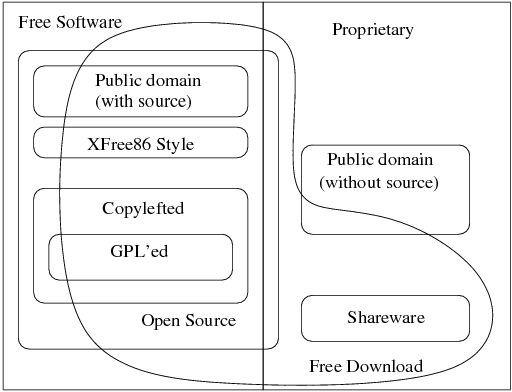
\includegraphics[scale=0.50,clip=true]{figs/venn.png}
% \end{center}
% \end{figure}

%\end{frame}




%%%%%%%%%%%%%%%%%%%%%%%%%%%%%%%%%%%%%%%%%%%%%%%%%%%%%%%%%%%%%%%%%%%%%%%
\begin{frame}
\frametitle{Permissible restrictions}
\begin{itemize}
    \item Attribution of authors (such attribution does not impede normal use of the work).
    \item Transmission of freedoms (copyleft or reciprocity).
    \item Protection of freedoms (access to source code or prohibition of ``technical measures'', DRM). 
\end{itemize}

\end{frame}

%%%%%%%%%%%%%%%%%%%%%%%%%%%%%%%%%%%%%%%%%%%%%%%%%%%%%%%%%%%%%%%%%%%%%%%
\begin{frame}
\frametitle{Warranty and disclaimer}
\begin{itemize}
    \item Software by itself is not a consumer product.
    \item When software is (combined into) a consumer product, disclaimers are ineffective.
    \item ``As Is'': we are accepting item in the actual state \textbf{with all faults}.
\end{itemize}

\end{frame}
 
%%%%%%%%%%%%%%%%%%%%%%%%%%%%%%%%%%%%%%%%%%%%%%%%%%%%%%%%%%%%%%%%%%%%%%%
\begin{frame}
\frametitle{BSD Disclaimer}

\begin{block}{BSD Warranty Disclaimer}
\small{THIS SOFTWARE IS PROVIDED BY THE COPYRIGHT HOLDERS AND CONTRIBUTORS ``AS IS'' AND ANY EXPRESS OR IMPLIED WARRANTIES, INCLUDING, BUT NOT LIMITED TO, THE IMPLIED WARRANTIES OF MERCHANTABILITY AND FITNESS FOR A PARTICULAR PURPOSE ARE DISCLAIMED. IN NO EVENT SHALL THE COPYRIGHT HOLDER OR CONTRIBUTORS BE LIABLE FOR ANY DIRECT, INDIRECT, INCIDENTAL, SPECIAL, EXEMPLARY, OR CONSEQUENTIAL DAMAGES (INCLUDING, BUT NOT LIMITED TO, PROCUREMENT OF SUBSTITUTE GOODS OR SERVICES; LOSS OF USE, DATA, OR PROFITS; OR BUSINESS INTERRUPTION) HOWEVER CAUSED AND ON ANY THEORY OF LIABILITY, WHETHER IN CONTRACT, STRICT LIABILITY, OR TORT (INCLUDING NEGLIGENCE OR OTHERWISE) ARISING IN ANY WAY OUT OF THE USE OF THIS SOFTWARE, EVEN IF ADVISED OF THE POSSIBILITY OF SUCH DAMAGE.}
\end{block}

\end{frame}



%%%%%%%%%%%%%%%%%%%%%%%%%%%%%%%%%%%%%%%%%%%%%%%%%%%%%%%%%%%%%%%%%%%%%%%

\begin{frame}
\frametitle{License compatibility}

\begin{itemize}
\item Two licenses are compatible if a joint derivate project could be delivered (i.e., the resulting code can be redistributed together).
\item Compatibility is determined by comparing restrictions imposed by each license.
\end{itemize}

Compatibility == merge source code from different FLOSS software licenses.

\end{frame}


%%%%%%%%%%%%%%%%%%%%%%%%%%%%%%%%%%%%%%%%%%%%%%%%%%%%%%%%%%%%%%%%%%%%%%%
\begin{frame}
\frametitle{Dual-licensing}

Distribute software under two different sets of terms and conditions. Motivations:

\begin{itemize}
\item License compatibility (Perl, Mozilla/Firefox, MySQL).
\item Market segregation based business models (MySQL Enterprise)
\item Allows the holder to offer customizations, early releases, generate other derivative works or grant rights to third parties to redistribute proprietary versions.
\end{itemize}

                                                 
\end{frame}


%%%%%%%%%%%%%%%%%%%%%%%%%%%%%%%%%%%%%%%%%%%%%%%%%%%%%%%%%%%%%%%%%%%%%%%
\begin{frame}
\frametitle{Proliferation of licenses}

\begin{itemize}
\item Vanity licenses: It has been a known problem in the community for a few years.
\item A growing number of licenses increases exponentially the possible combinations and interactions. 
\item This fact makes it difficult to merge code from diverse sources, both for incompatibility issues and unacceptable clauses.
\item It introduces juridical insecurity requiring lawyers, that it is what free licenses where trying to avoid in the first place (i.e. the EUPL license and EULAs).
\item It favors FUD (Fear, Uncertainly, Doubt).
\end{itemize}                                                 

\end{frame}

%%%%%%%%%%%%%%%%%%%%%%%%%%%%%%%%%%%%%%%%%%%%%%%%%%%%%%%%%%%%%%%%%%%%%%%

\subsection{Software Patents}

%%%%%%%%%%%%%%%%%%%%%%%%%%%%%%%%%%%%%%%%%%%%%%%%%%%%%%%%%%%%%%%%%%%%%%%
\begin{frame}
\frametitle{Patents. Concepts}

\begin{itemize}
\item \alert{Exclusive rights} (monopoly) granted by a sovereign state to an inventor for a limited period of time in exchange for the \alert{public disclosure} of an \alert{invention}.
	\begin{itemize}
	\item Industrial fields: devices or processes that perform a practical (``useful'') function
	\item Novelty (no ``prior art'')
	\item Non-obviousness
	\end{itemize}                                                 
\item Certain subject areas can be excluded: business methods and computer programs.
\item Philosophical, mathematical or scientific discoveries cannot be protected.
\end{itemize}                                                 

\end{frame}



%%%%%%%%%%%%%%%%%%%%%%%%%%%%%%%%%%%%%%%%%%%%%%%%%%%%%%%%%%%%%%%%%%%%%%%

\begin{frame}
\frametitle{Software patents}

\begin{columns}

\column[t]{6.5cm}


\begin{itemize}
\item Definition disputed.
\item Intense and active debate for years.
\item European Union: article 52 (European Patent Convention) excludes ``programs for computers \alert{as such}''. 
\item Japan: Software-related inventions are patentable.
\item USA: software patents allowed.
\end{itemize}


\column[t]{5cm}

\begin{figure}
 \vspace{0.3cm}
\begin{flushleft}
	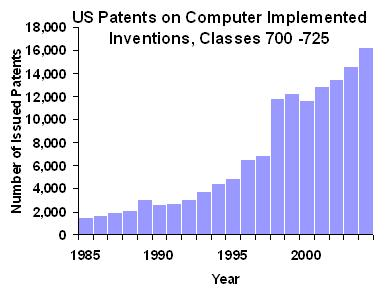
\includegraphics[scale=0.5,clip=true]{figs/Software_patents2.JPG}
\end{flushleft}
\end{figure}

\end{columns}

\end{frame}

%%%%%%%%%%%%%%%%%%%%%%%%%%%%%%%%%%%%%%%%%%%%%%%%%%%%%%%%%%%%%%%%%%%%%%%
\begin{frame}
\frametitle{Software patents}

\begin{itemize}
\item Europe: Although not legal, in
  practice, lots of algorithms, and in fact, ideas, have been
  patented.
\item Since trivial ideas (implemented with algorithms) are patented,
  they are often used by owners to drown competitors.
\item It is very easy to infringe a lot of patents when developing a software project.
\item ``\alert{Patent trolls}'': patent owner who doesn't manufacture or use the patented invention, but it seeks to enforce its right through the negotiation of licenses and litigation.
Also known as \alert{Non-Practicing Entity} (NPE).
\item PatentFreedom.com provides updated information about patent trolls and NPEs.
\end{itemize}

\end{frame}

%%%%%%%%%%%%%%%%%%%%%%%%%%%%%%%%%%%%%%%%%%%%%%%%%%%%%%%%%%%%%%%%%%%%%%%

\begin{frame}
\frametitle{Patent trolls - NPE}

\begin{figure}
 \vspace{-0.3cm}
\begin{center}
	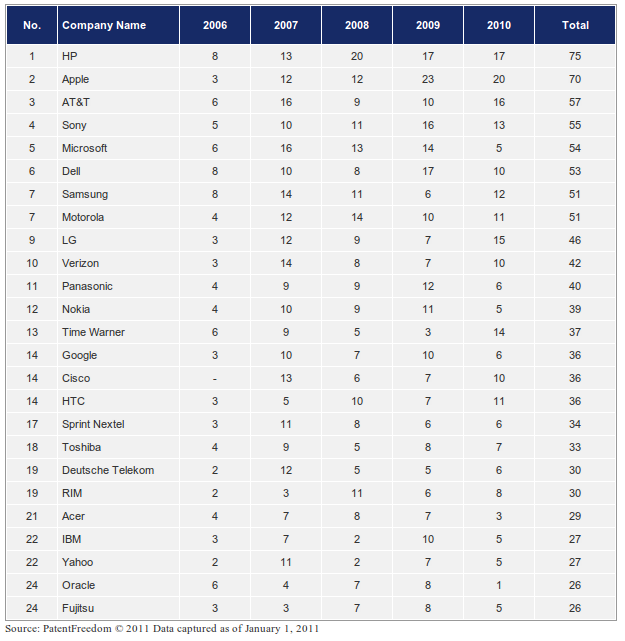
\includegraphics[scale=0.35,clip=true]{figs/patent-trolls.png}
\end{center}
\end{figure}

\end{frame}


%%%%%%%%%%%%%%%%%%%%%%%%%%%%%%%%%%%%%%%%%%%%%%%%%%%%%%%%%%%%%%%%%%%%%%%
\begin{frame}
\frametitle{Patents: Incentive for software innovation?}

A reason for its existence is that it encourages inventions to be shared rather than be kept secret. Is it true with software?

\pause

\begin{itemize}
\item The academic community publishes their innovations to the public.
\item There is a massive and rapidly growing amount of innovative open source software.
\item Companies have strong incentives to participate in open source.
\end{itemize}

\end{frame}


%%%%%%%%%%%%%%%%%%%%%%%%%%%%%%%%%%%%%%%%%%%%%%%%%%%%%%%%%%%%%%%%%%%%%%%
\begin{frame}
\frametitle{Software patents}

\begin{itemize}
\item The patent system doesn't exist to protect intellectual property.
\item The patent system exists to provide an incentive for innovation \textit{where that incentive would not have existed otherwise}.
\item If the incentive to create the innovation was there without the patent system, then the patent system is serving no purpose.
\end{itemize}

\end{frame}

%%%%%%%%%%%%%%%%%%%%%%%%%%%%%%%%%%%%%%%%%%%%%%%%%%%%%%%%%%%%%%%%%%%%%%%
\begin{frame}
\frametitle{Software patents}

Do patents encourage innovation in startups by protecting them from having their ideas ``stolen''?

\pause

\begin{itemize}
\item Patents are a cost.
\item Startups must build ``defensive patent portfolios''.
\end{itemize}

\end{frame}

%%---------------------------------------------------------------
%%%%%%%%%%%%%%%%%%%%%%%%%%%%%%%%%%%%%%%%%%%%%%%%%%%%%%%%%%%%%%%%%%%%%%%
% \section{References}
%%%%%%%%%%%%%%%%%%%%%%%%%%%%%%%%%%%%%%%%%%%%%%%%%%%%%%%%%%%%%%%%%%%%%%%

\begin{frame}
\frametitle{References}

\begin{itemize}
\item \textsc{Van Lindberg}, \textit{Intellectual Property and Open Source}, O'Reilly, July 2008.
\item \textsc{Malcolm Bain} et al. \textit{Aspectos legales y de explotación del software libre}, UOC, February 2007. \\
\url{http://ocw.uoc.edu/informatica-tecnologia-y-multimedia/aspectos-legales-y-de-explotacion-del-software-libre/materiales/}
\item \textsc{Lawrence Rose}, \textit{Open Source Licensing}, Prentice Hall, July 2004 
\end{itemize}

\end{frame}


%%%%%%%%%%%%%%%%%%%%%%%%%%%%%%%%%%%%%%%%%%%%%%%%%%%%%%%%%%%%%%%%%%%%%%%



